\section{滑轮}\label{sec:7-5}

滑轮是各种起重设备中常见的简单机械。图 \ref{fig:7-19} 的照片是正在利用滑轮吊起内燃机车准备装船的情形。
现在我们来研究使用滑轮有什么好处和怎样使用滑轮。

\begin{figure}[htbp]
    \centering
    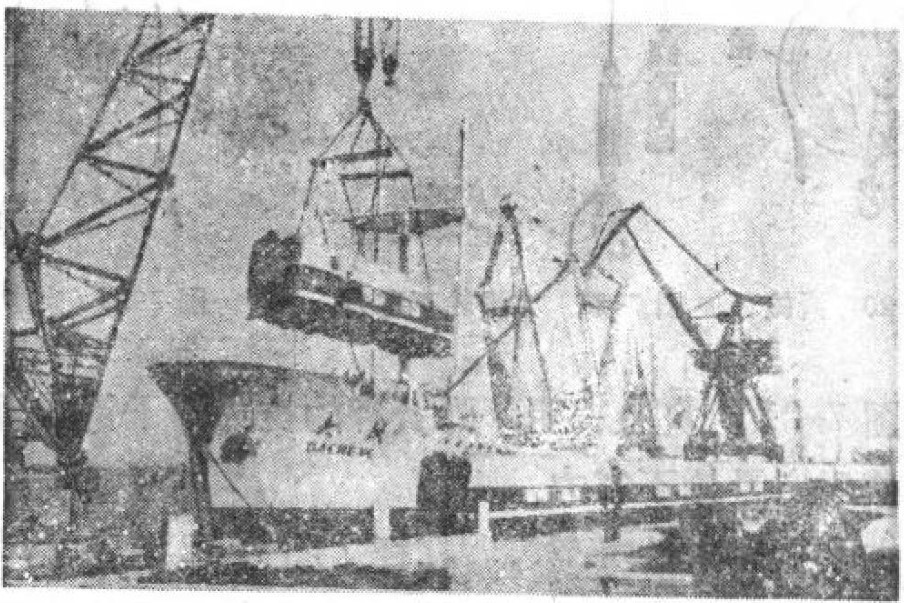
\includegraphics[width=0.7\textwidth]{../pic/czwl1-ch7-19}
    \caption{}\label{fig:7-19}
\end{figure}


(1) 定滑轮

你见过升旗吗?升旗的人向下拉绳,旗子就上升。
旗子运动的方向同人拉绳的方向相反,是因为旗杆顶上安装着一个小滑轮。

滑轮是一个周边有槽的小轮(图 \ref{fig:7-20}),可以绕着装在框子里的轴转动。
象图 \ref{fig:7-21} 那样使用滑轮,滑轮的轴固定不动,我们把这样的滑轮叫\textbf{定滑轮}。

\begin{figure}[htbp]
    \centering
    \begin{minipage}{4cm}
    \centering
    \vspace{6em}
    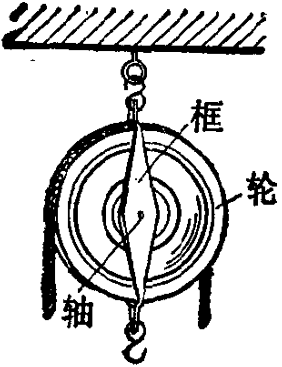
\includegraphics[width=3cm]{../pic/czwl1-ch7-20}
    \caption{滑轮}\label{fig:7-20}
    \end{minipage}
    \qquad
    \begin{minipage}{5cm}
    \centering
    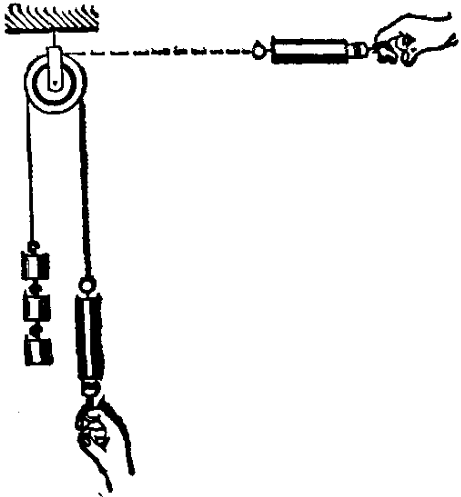
\includegraphics[width=5cm]{../pic/czwl1-ch7-21}
    \caption{定滑轮不省力}\label{fig:7-21}
    \end{minipage}
    \qquad
    \begin{minipage}{4cm}
    \centering
    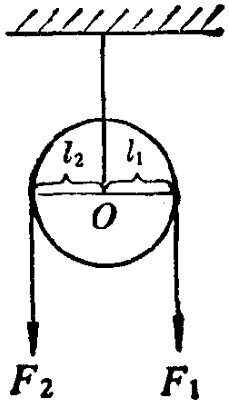
\includegraphics[width=3cm]{../pic/czwl1-ch7-22}
    \caption{定滑轮相当于等臂杠杆}\label{fig:7-22}
    \end{minipage}
\end{figure}

图 \ref{fig:7-21} 的实验表明,弹簧秤的拉力等于钩码重,可见使用定滑轮不省力。

\CJKunderwave{定滑轮实质是一个等臂杠杆}。
图 \ref{fig:7-22} 是定滑轮的杠杆示意图,动力臂 $l_1$、阻力臂 $l_2$ 都等于滑轮半径。
根据杠杆平衡条件,也可以得出使用定滑轮不省力的结论。

\CJKunderwave{使用定滑轮虽然不省力,但是可以改变力的方向}。
在许多情形下,改变力的方向对我们是很方便的。
比如,旗杆顶上装一个定滑轮,人站在地上就能把旗子升到高处。在提升不太重的物体时,常常使用定滑轮。

(2) 动滑轮

我们可以照图 \ref{fig:7-23} 那样使用滑轮,在高处拉绳子的一端,将滑轮和它下面挂的物体一起提上来。
这样使用滑轮的时候,滑轮和重物一起移动,我们把这样的滑轮叫\textbf{动滑轮}。

\begin{figure}[htbp]
    \centering
    \begin{minipage}{3.5cm}
    \centering
    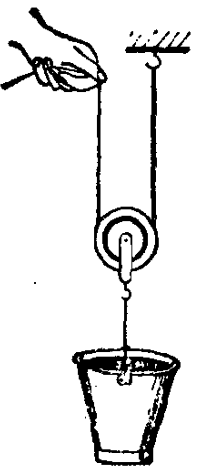
\includegraphics[width=3cm]{../pic/czwl1-ch7-23}
    \caption{动滑轮}\label{fig:7-23}
    \end{minipage}
    \qquad
    \begin{minipage}{5cm}
    \centering
    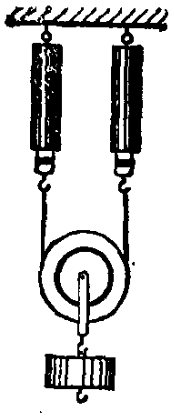
\includegraphics[width=3cm]{../pic/czwl1-ch7-24}
    \caption{}\label{fig:7-24}
    \end{minipage}
    \qquad
    \begin{minipage}{5cm}
    \centering
    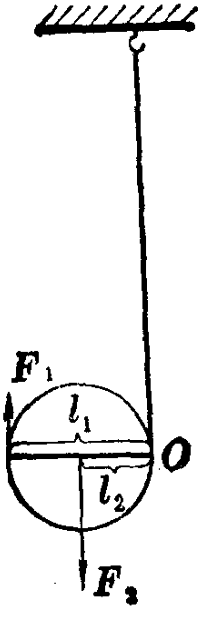
\includegraphics[width=3cm]{../pic/czwl1-ch7-25}
    \caption{动滑轮相当动力臂是阻力臂二倍的杠杆}\label{fig:7-25}
    \end{minipage}
\end{figure}

使用动滑轮有什么好处呢?

图 \ref{fig:7-24} 的实验表明,两个弹簧秤的拉力相同,并且这两个拉力之和等于动滑轮和钩码的总重。
这就是说,使用动滑轮的时候,每段绳子只承担物体重的一半。所以\CJKunderwave{使用动滑轮省一半力}。

从图 \ref{fig:7-25} 可以看出,\CJKunderwave{动滑轮实质是动力臂($l_1$)为阻力臂($l_2$)二倍的杠杆},
根据杠杆平衡条件可以知道,动力 $F_1$ 是阻力 $F_2$ 的一半,即同样得出使用动滑轮能省一半力的结论。

使用动滑轮能省一半力,但是不能改变力的方向,在很多情况下是不方便的,因此动滑轮很少单独使用。

(3) 滑轮组

实际应用滑轮的时候,常常既要求省力,又要求方便。
由于动滑轮能省力,定滑轮能改变力的方向,所以把它们组合起来使用(图 \ref{fig:7-26}),
就能既省力,又方便。


\begin{figure}[htbp]
    \centering
    \begin{minipage}{7cm}
    \centering
    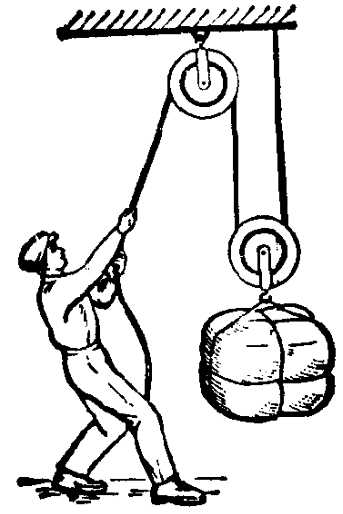
\includegraphics[width=5cm]{../pic/czwl1-ch7-26}
    \caption{滑轮组}\label{fig:7-26}
    \end{minipage}
    \qquad
    \begin{minipage}{7cm}
    \centering
    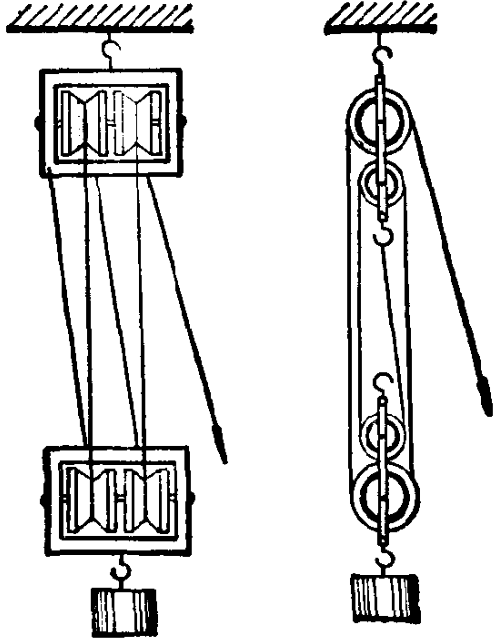
\includegraphics[width=6cm]{../pic/czwl1-ch7-27}
    \caption{四个滑轮组成的滑轮组}\label{fig:7-27}
    \end{minipage}
\end{figure}


动滑轮和定滑轮组合在一起叫\textbf{滑轮组}。

图 \ref{fig:7-27} 所示的是由四个滑轮组成的滑轮组。
上面两个定滑轮装在一个框子里,下面两个动滑轮装在一个框子里,
绳子的一端拴在定滑轮上,然后依次绕过动滑轮和定滑轮,力加在绳子的另一端上。
在这样的滑轮组里,重物和动滑轮的总重由四段绳子承担,每段绳子承担总重的四分之一。
所以用这样的滑轮组提起重物,用的力只是总重的四分之一。

\textbf{使用滑轮组的时候,重物和动滑轮的总重由几段绳子承担,提起重物所用的力就是总重的几分之一}。

前面的分析都省略了滑轮和轴之间的摩擦,所以在使用定滑轮、动滑轮和滑轮组的时候,实际用的力都比前面所讲的要大一些。



\nonumsection{阅读材料:起重机}

你见过起重机(也叫吊车)吗?
如果你是在现代化的建筑工地上看到过,你可能亲眼看过它把成吨的建筑器材提到几十米的高处。
如果你是在现代化的港口码头看到过,你可能亲眼看过它把几十吨的货物提上几十米高的轮船甲扳。
你知道吗?在大型造船厂,起重机能把上百吨的发动机吊到几百米外的船体中去。

由于起重机有很多用处,起重机的种类也很多。不同的起重机有不同的结构特征和起重性能,
但是它们都是由简单机械组合发展来的。

图 \ref{fig:7-28} 是一台汽车起重机的示意图。
起重钩的升降是靠由 $A$、$B$ 组成的滑轮组的作用,
滑轮组钢丝绳的收放是靠装在 $C$ 里的卷扬机(轮轴)的作用,
起重臂围绕 $O$ 的起伏是靠杆 $E$ 伸出或缩进 $D$ 的作用,起重臂是个杠杆。


\begin{figure}[htbp]
    \centering
    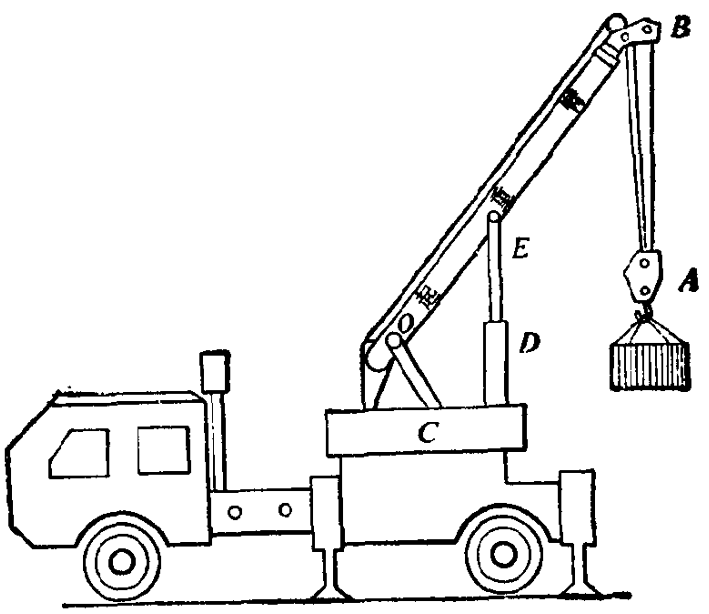
\includegraphics[width=0.5\textwidth]{../pic/czwl1-ch7-28}
    \caption{汽车起重机}\label{fig:7-28}
\end{figure}


\lianxi

解下列各题时,都不考虑摩擦力。

(1) 用图 \ref{fig:7-23} 的动滑轮提起 150 牛顿的灰桶。挂灰桶的绳子承受多大的力?
人拉绳子要用多大的力?不计动滑轮本身重。

(2) 用图 \ref{fig:7-26} 的滑轮组提起货物,动滑轮重 20 牛顿,所用的拉力是 210 牛顿,求货物重多少。

(3) 一根绳子只能支持 3000 牛顿的力。使用滑轮组能不能用这根绳子提起重 $10^4$ 牛顿的物体?
应当怎样装配才行?不计动滑轮本身重。

(4) 图 \ref{fig:7-29} 是一种塔式起重机的起重滑轮组,它是由一个动滑轮和两个定滑轮组成的。
假如我们把钢丝绳照图甲、乙、丙那样绕在滑轮上,那么每种绕法中起作用的滑轮是哪几个?
哪种绕法最省力?为什么?
如果钢丝绳只能支持 $10^4$ 牛顿的力,那么这三种绕法能吊起的最大重力各是多少?
不计动滑轮本身重。

\begin{figure}[htbp]
    \centering
    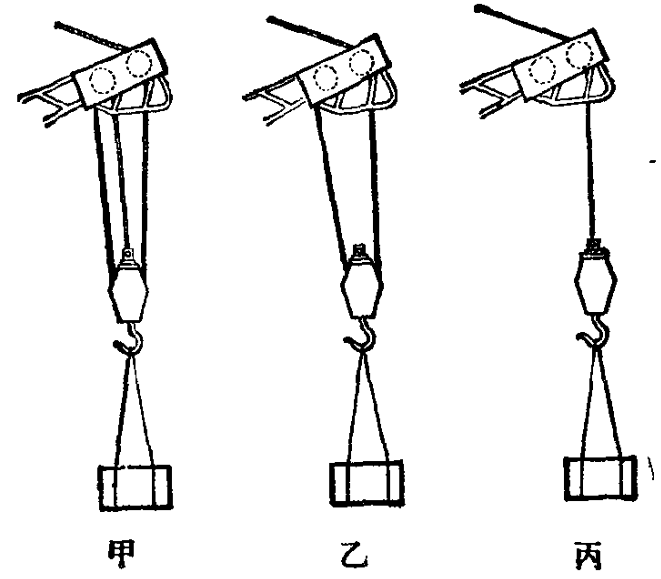
\includegraphics[width=0.5\textwidth]{../pic/czwl1-ch7-29}
    \caption{}\label{fig:7-29}
\end{figure}


